
\documentclass[11pt]{article}
\usepackage[letterpaper, margin=1in]{geometry}

% Used to place appendix in the toc with proper titles
\usepackage[toc,page,title]{appendix}
\renewcommand{\appendixname}{Appendix} % Used to rename from "Appendices" to "Appendix"
\renewcommand{\appendixpagename}{Appendix} % Used to rename from "Appendices" to "Appendix"
\renewcommand{\appendixtocname}{Appendix} % Used to rename from "Appendices" to "Appendix"

% Used to make citations/bibliography
% Usage:
% \bibliography{./bibliography/fullbib.bib}
% \bibliographystyle{plain}
\usepackage{cite}

% To enable forcing figure placement
\usepackage{float}

% Used to skip to next paragraph when a blank line is used between sentences
\usepackage{parskip}

% Used to change line spacing (double spaced, 1.5, etc.)
% Usage: 
% \begin{spacing}{1.5}
% \end{spacing}
\usepackage{setspace}

% Used for inserting images.
% Usage: 
% \begin{figure}[hpt]
%     \centering
%     \caption{Caption}
%     \includegraphics[width=0.6\textwidth]{images/<IMG.NAME>}
%     \label{fig:<LABEL>}
% \end{figure}
\usepackage{graphicx}
\graphicspath{ {./images/} }

% Subplots
\usepackage{subcaption}

% Used for in text code with formatting and language highlighting
\usepackage{listings}
\usepackage{xcolor}

\usepackage[breaklinks]{hyperref}
\usepackage{url}

% Define custom style
\lstdefinestyle{mystyle}{
    basicstyle=\ttfamily\footnotesize, % Use a monospaced font with strict sizing
    numbers=left, % Show line numbers
    numbersep=5pt,
    numberstyle=\tiny\color{gray},
    stepnumber=1, % Ensures every line gets numbered
    tabsize=4, % Set tab width
    keepspaces=true, % Preserve spaces
    showspaces=false,
    showstringspaces=false,
    breaklines=true,
    breakatwhitespace=false,
    columns=fixed, % Maintain strict spacing
    lineskip=-1pt, % Prevent additional spacing between lines
    frame=single, % Optional: adds a border around the code
    rulecolor=\color{black},
    backgroundcolor=\color{white},
    keywordstyle=\color{blue}\bfseries, % Style for keywords
    stringstyle=\color{red}, % Style for strings
    commentstyle=\color{gray}, % Style for comments
    xleftmargin=5pt, % Adjusts left margin outside the frame
    xrightmargin=5pt % Adjusts right margin outside the frame
}
\renewcommand{\lstlistingname}{Code Block}


\lstset{style=mystyle}

% Used to create hyperlink references that can be clicked within the PDF
% Usage: \ref{<SECTIONLABEL>}
\usepackage{hyperref}

% Used for certain math symbols
\usepackage{amssymb}

\usepackage{array}
\usepackage{ragged2e}

\usepackage{titlesec}
\usepackage{bookmark}

\setlength\parindent{0pt}

\title{%
  ELEC 873 \\
Assignment 1}

\author{Anthony Sicoie (20214793)}

\begin{document}

\maketitle

\section*{Preamble}

For each question code was developed locally and tested on both my machine (Ryzen 9 7950x, 64 GD Ram) as well as the KNL server.
The code was built using makefiles following a similar format to the one present in Code Block \ref{a:make} of the appendix.
This is the Makefile template that all questions also followed, with appropriate changes based on the question requirements for each one; where questions only required a single implementation (only OpenMP etc.), only that implementation was accounted for in.
Furthermore, the Makefile was also used to run the code in all cases other than those utilizing bash scripts; in those cases it is mentioned explicitly.
Comments are provided throughout the Code Blocks for any noteworthy or special conditions I felt were worth highlighting.
As such discussion of code within the report is minimal, but rather the comments are intended to describe how the code functions.


\section*{Q1:}

Code Blocks \ref{q1:mpi}, \ref{q1:openmp}, and \ref{q1:pthread} present the question 1 code using MPI, OpenMP, and Pthreads respectively to print basic "Hello World" messages.
The output of the code can be found in the Figure \ref{fig:q1}.
All code was run with 8 processes/threads, though any number can be set via the \texttt{Makefile} \texttt{make runall n=<number\_of\_threads/processes>} directive. 
This can be seen in the Code Block \ref{a:make} of the appendix where the Makefile code is provided.

\lstinputlisting[language=C, caption=\centering{MPI code for question 1}, label={q1:mpi}]{../q1/mpi.c}
\lstinputlisting[language=C, caption=\centering{OpenMP code for question 1}, label={q1:openmp}]{../q1/openmp.c}
\lstinputlisting[language=C, caption=\centering{Pthread code for question 1}, label={q1:pthread}]{../q1/pthread.c}


\begin{figure}[H]
\centering
    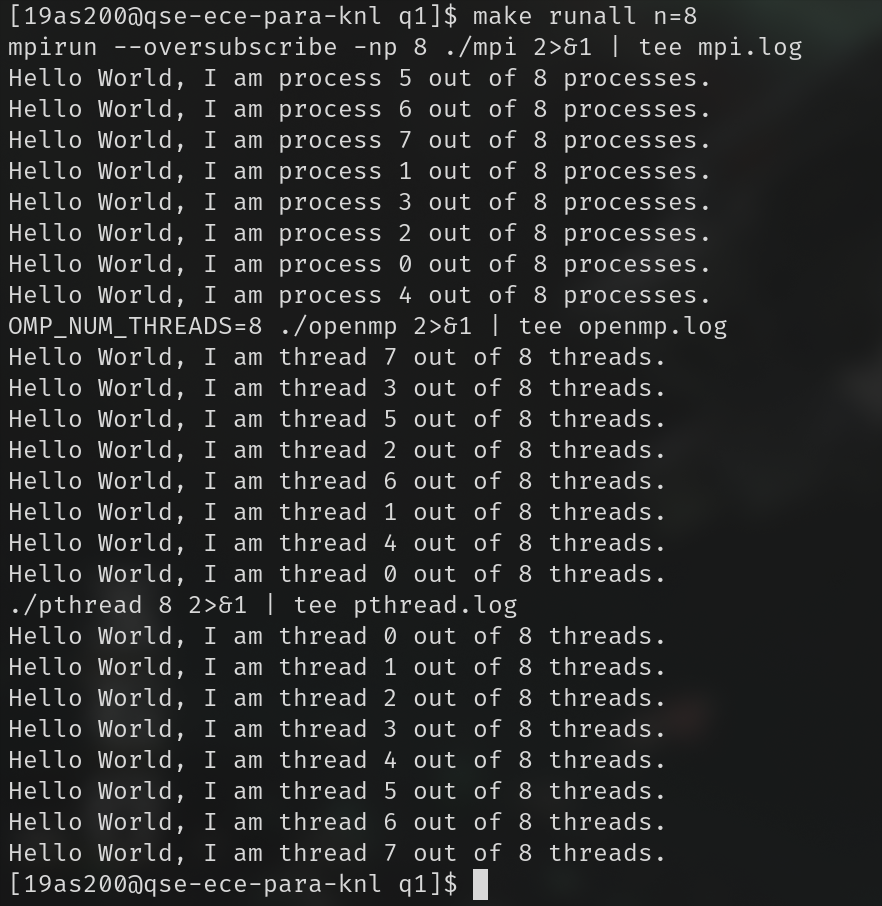
\includegraphics[width=0.4\textwidth]{./images/q1.png}
\caption{Output for question 1}
\label{fig:q1}
\end{figure}

\newpage

\section*{Q2:}

Code Blocks \ref{q2:mpi}, \ref{q2:openmp}, and \ref{q2:pthread} present the question 2 code using MPI, OpenMP, and Pthreads respectively to compute \textit{pi}.
The output of the code can be found in the Figure \ref{fig:q2}.
All code was run with 8 processes/threads, though any number can be set. 

\lstinputlisting[language=C, caption=\centering{MPI code for question 2}, label={q2:mpi}]{../q2/mpi.c}
\lstinputlisting[language=C, caption=\centering{OpenMP code for question 2}, label={q2:openmp}]{../q2/openmp.c}
\lstinputlisting[language=C, caption=\centering{Pthread code for question 2}, label={q2:pthread}]{../q2/pthread.c}


\begin{figure}[H]
\centering
    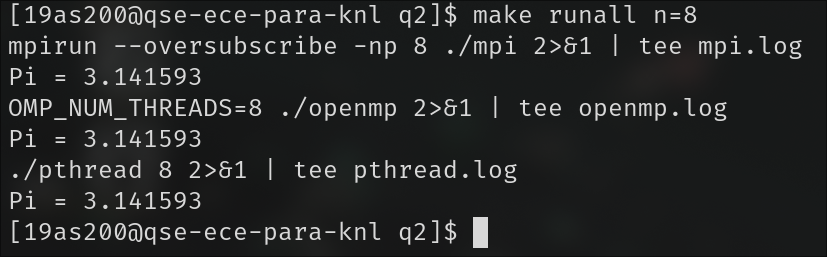
\includegraphics[width=\textwidth]{./images/q2.png}
\caption{Output for question 2}
\label{fig:q2}
\end{figure}

\newpage
\section*{Q3:}
Code Block \ref{q3:openmp} presents the question 3 code using OpenMP to compute the sum of 1000 numbers.
The output of the code can be found in the Figure \ref{fig:q3}.
The Code was run with 8 threads, but is modular and functions with any number of threads due to how OpenMP automatically handles multithreading.

\lstinputlisting[language=C, caption=\centering{OpenMP code for question 3}, label={q3:openmp}]{../q3/openmp.c}

\begin{figure}[H]
\centering
    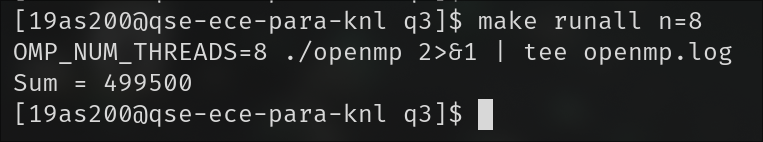
\includegraphics[width=\textwidth]{./images/q3.png}
\caption{Output for question 3}
\label{fig:q3}
\end{figure}

\newpage
\section*{Q4:}
Code Block \ref{q4:mpi} presents the question 4 code using MPI to perform send operations in a unidirectional ring of 8 processes.
The output of the code can be found in the Figure \ref{fig:q4}, however it is worth noting that the code is modular and can function with more or less than 8 processes due to the way the variable \texttt{size} set by \texttt{MPI\_Comm\_Size} was utilized.
The code was run with 8 processes and leverages \texttt{MPI\_Send/Recv} functions to arbitrate communication; notably, process 0 waits until it receives the last message from process $n-1$ before exiting.

\lstinputlisting[language=C, caption=\centering{MPI code for question 4}, label={q4:mpi}]{../q4/mpi.c}

\begin{figure}[H]
\centering
    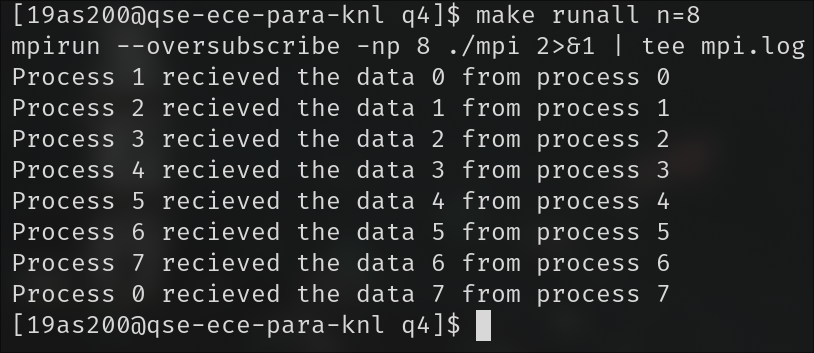
\includegraphics[width=0.5\textwidth]{./images/q4.png}
\caption{Output for question 4}
\label{fig:q4}
\end{figure}

\newpage

\section*{Q5:}

Code Block \ref{q5:mpi} presents the question 5 code using MPI to represent a 3D Mesh; this is done through the use of the \texttt{MPI\_Cart\_create} function primarily, and assumes that a 2D plane in 3D is equivalent to a row in 2D.
The output of the code can be found in Figure \ref{fig:q5}, however it is worth noting that the code is modular and can function with more than 8 processes so long as they are cubes as this was accounted for through the use of the \texttt{size} variable.
The code was run with 8 processes in the example, therefore there are two planes present.

\lstinputlisting[language=C, caption=\centering{MPI code for question 5}, label={q5:mpi}]{../q5/mpi.c}

\begin{figure}[H]
\centering
    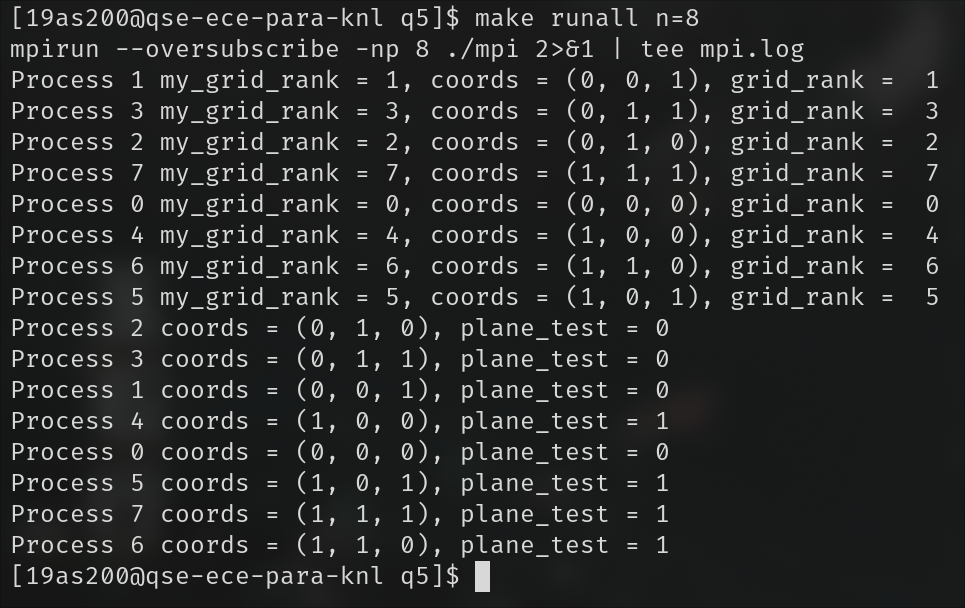
\includegraphics[width=\textwidth]{./images/q5.png}
\caption{Output for question 5}
\label{fig:q5}
\end{figure}

\newpage

\section*{Q6:}

Code Block \ref{q6:mpi} presents the question 6 code using MPI to do a ring-based scatter leveraging \texttt{MPI\_Pack} and \texttt{MPI\_Unpack}.
The output for the code can be found in Figure \ref{fig:q6}.
The code leverages the \texttt{size} variable to detect the size of the comm and function beyond the 8 processes initially required.
The code was run for demonstrative purposes utilizing 8 processes, packing and unpacking an array that is filled via a for loop where each process expects to receive $own\ rank + 1$ as the data it retains.

\lstinputlisting[language=C, caption=\centering{MPI code for question 6}, label={q6:mpi}]{../q6/mpi.c}

\begin{figure}[H]
\centering
    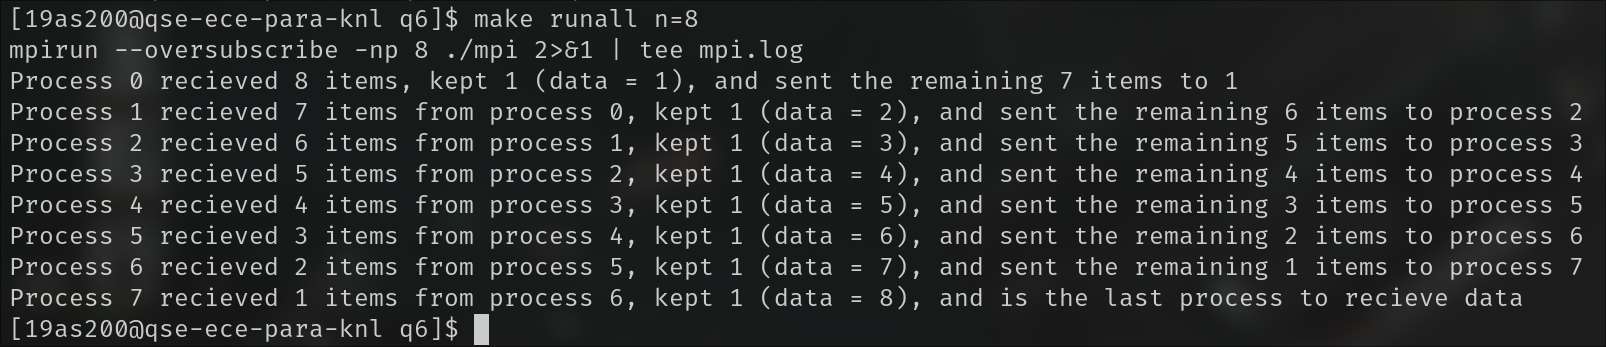
\includegraphics[width=\textwidth]{./images/q6.png}
\caption{Output for question 6}
\label{fig:q6}
\end{figure}

\newpage
\section*{Q7:}

Code Blocks \ref{q7:mpi}, \ref{q7:openmp}, \ref{q7:pthread}, and \ref{q7:hybrid} present the question 7 code using MPI, OpenMP, Pthreads, and a Hybrid MPI+OpenMP implementation respectively to find the min in an array.
Of note is the hybrid code, which allows the user to vary the array size via a command line argument and also handles timing as explained in the Analysis Sub Section.

\lstinputlisting[language=C, caption=\centering{MPI code for question 7}, label={q7:mpi}]{../q7/mpi.c}
\lstinputlisting[language=C, caption=\centering{OpenMP code for question 7}, label={q7:openmp}]{../q7/openmp.c}
\lstinputlisting[language=C, caption=\centering{Pthread code for question 7}, label={q7:pthread}]{../q7/pthread.c}
\lstinputlisting[language=C, caption=\centering{Hybrid (MPI+OpenMP) code for question 7}, label={q7:hybrid}]{../q7/hybrid.c}

\subsection*{Analysis:}

\begin{figure}[H]
\centering
\begin{subfigure}[t]{0.48\textwidth}
  \centering
    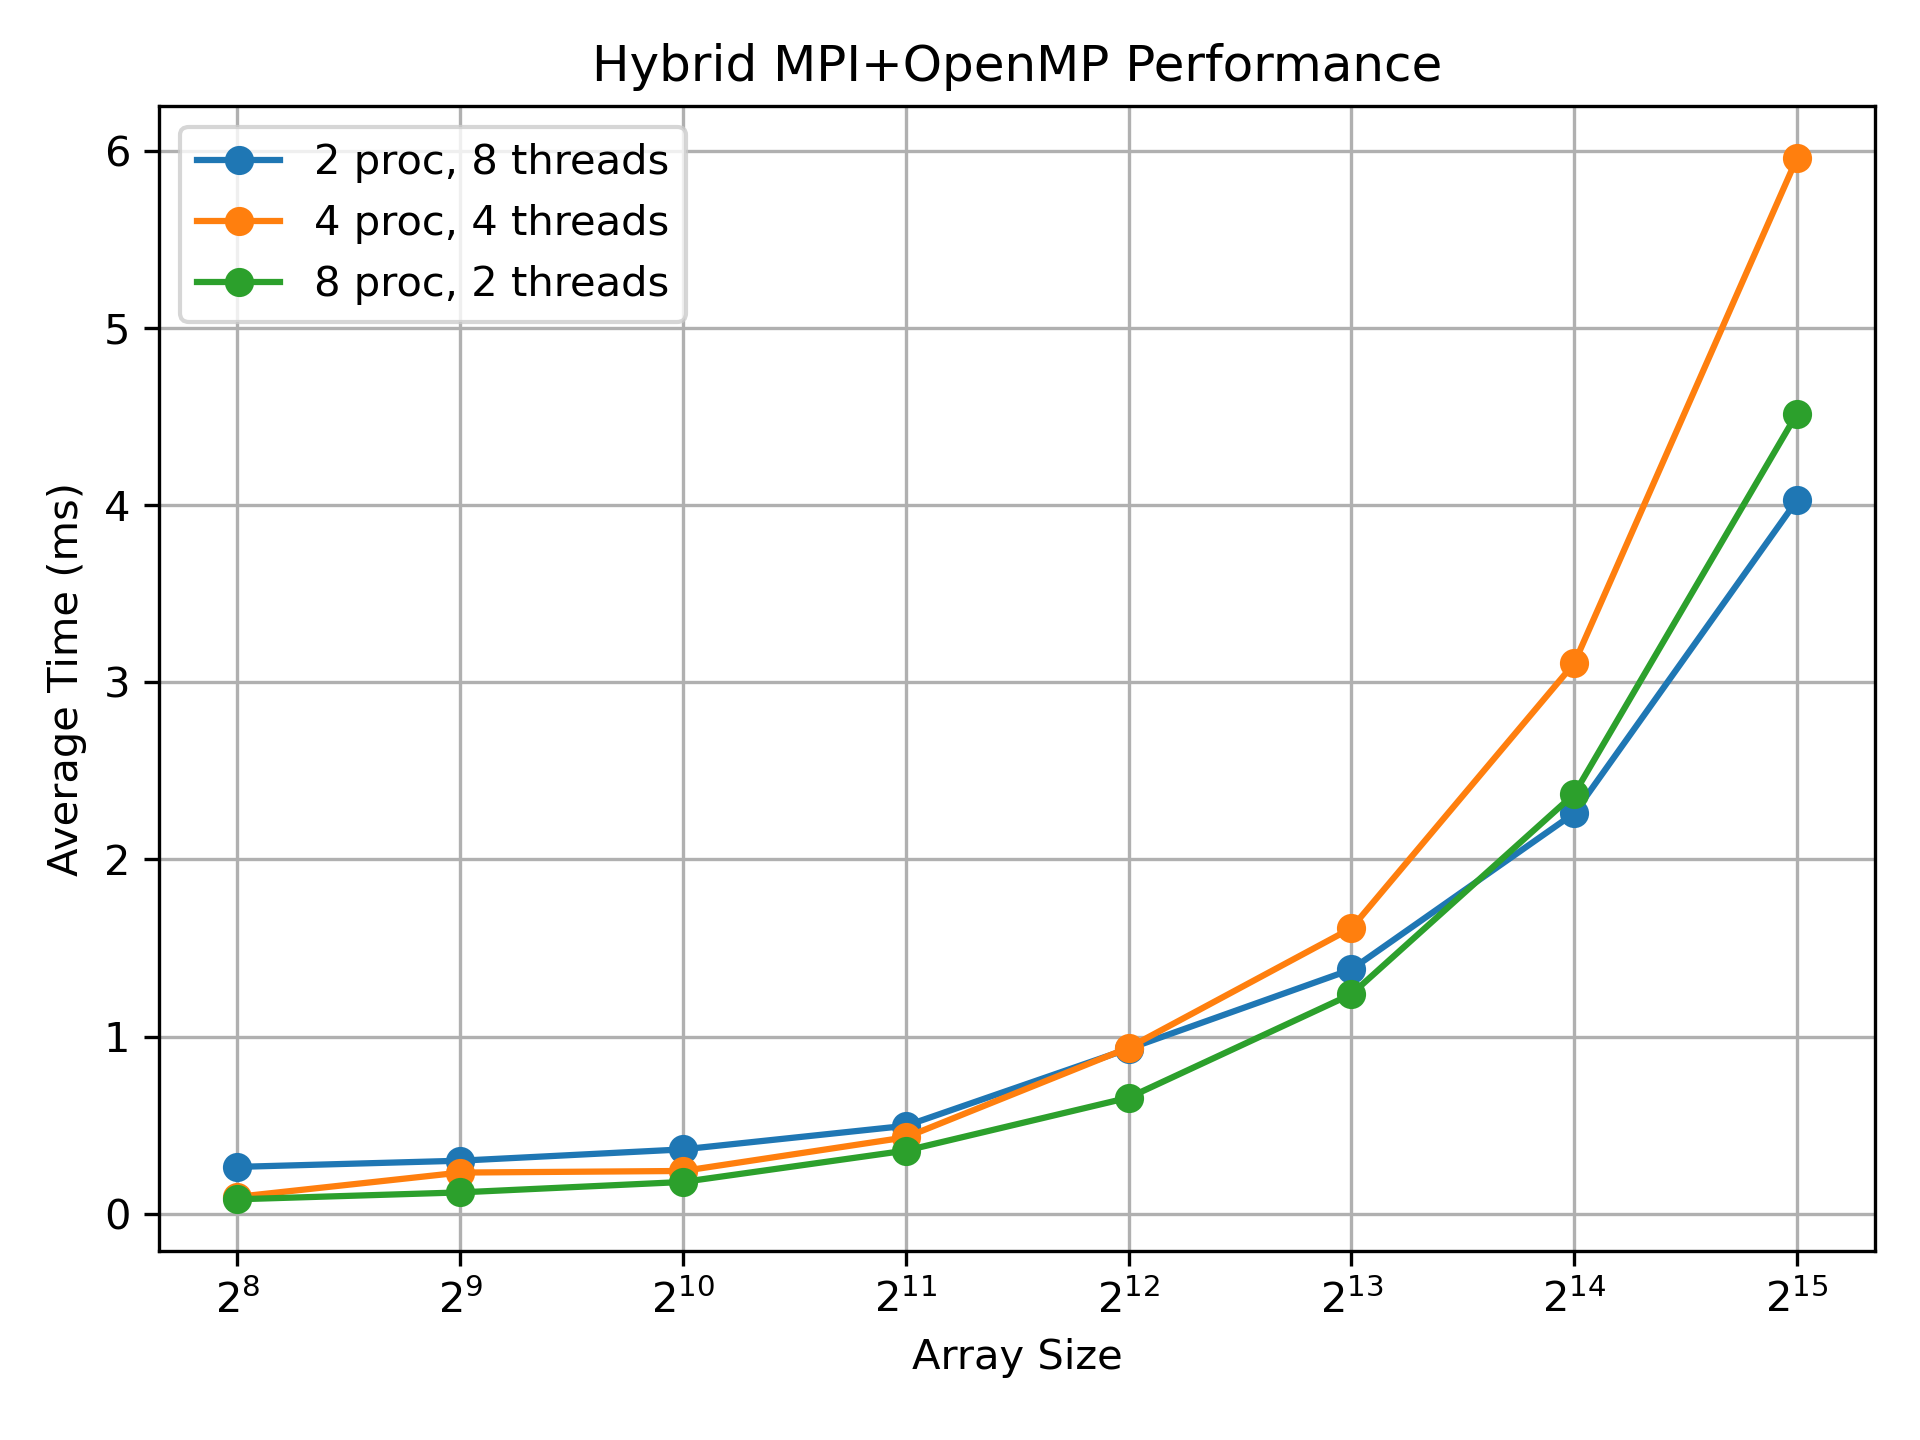
\includegraphics[width=\textwidth]{./images/knlq7.png}
  \caption{Varied process$\times$thread configurations run on the KNL server}\label{fig:knlq7}
\end{subfigure}%
\hfill
\begin{subfigure}[t]{0.48\textwidth}
  \centering
    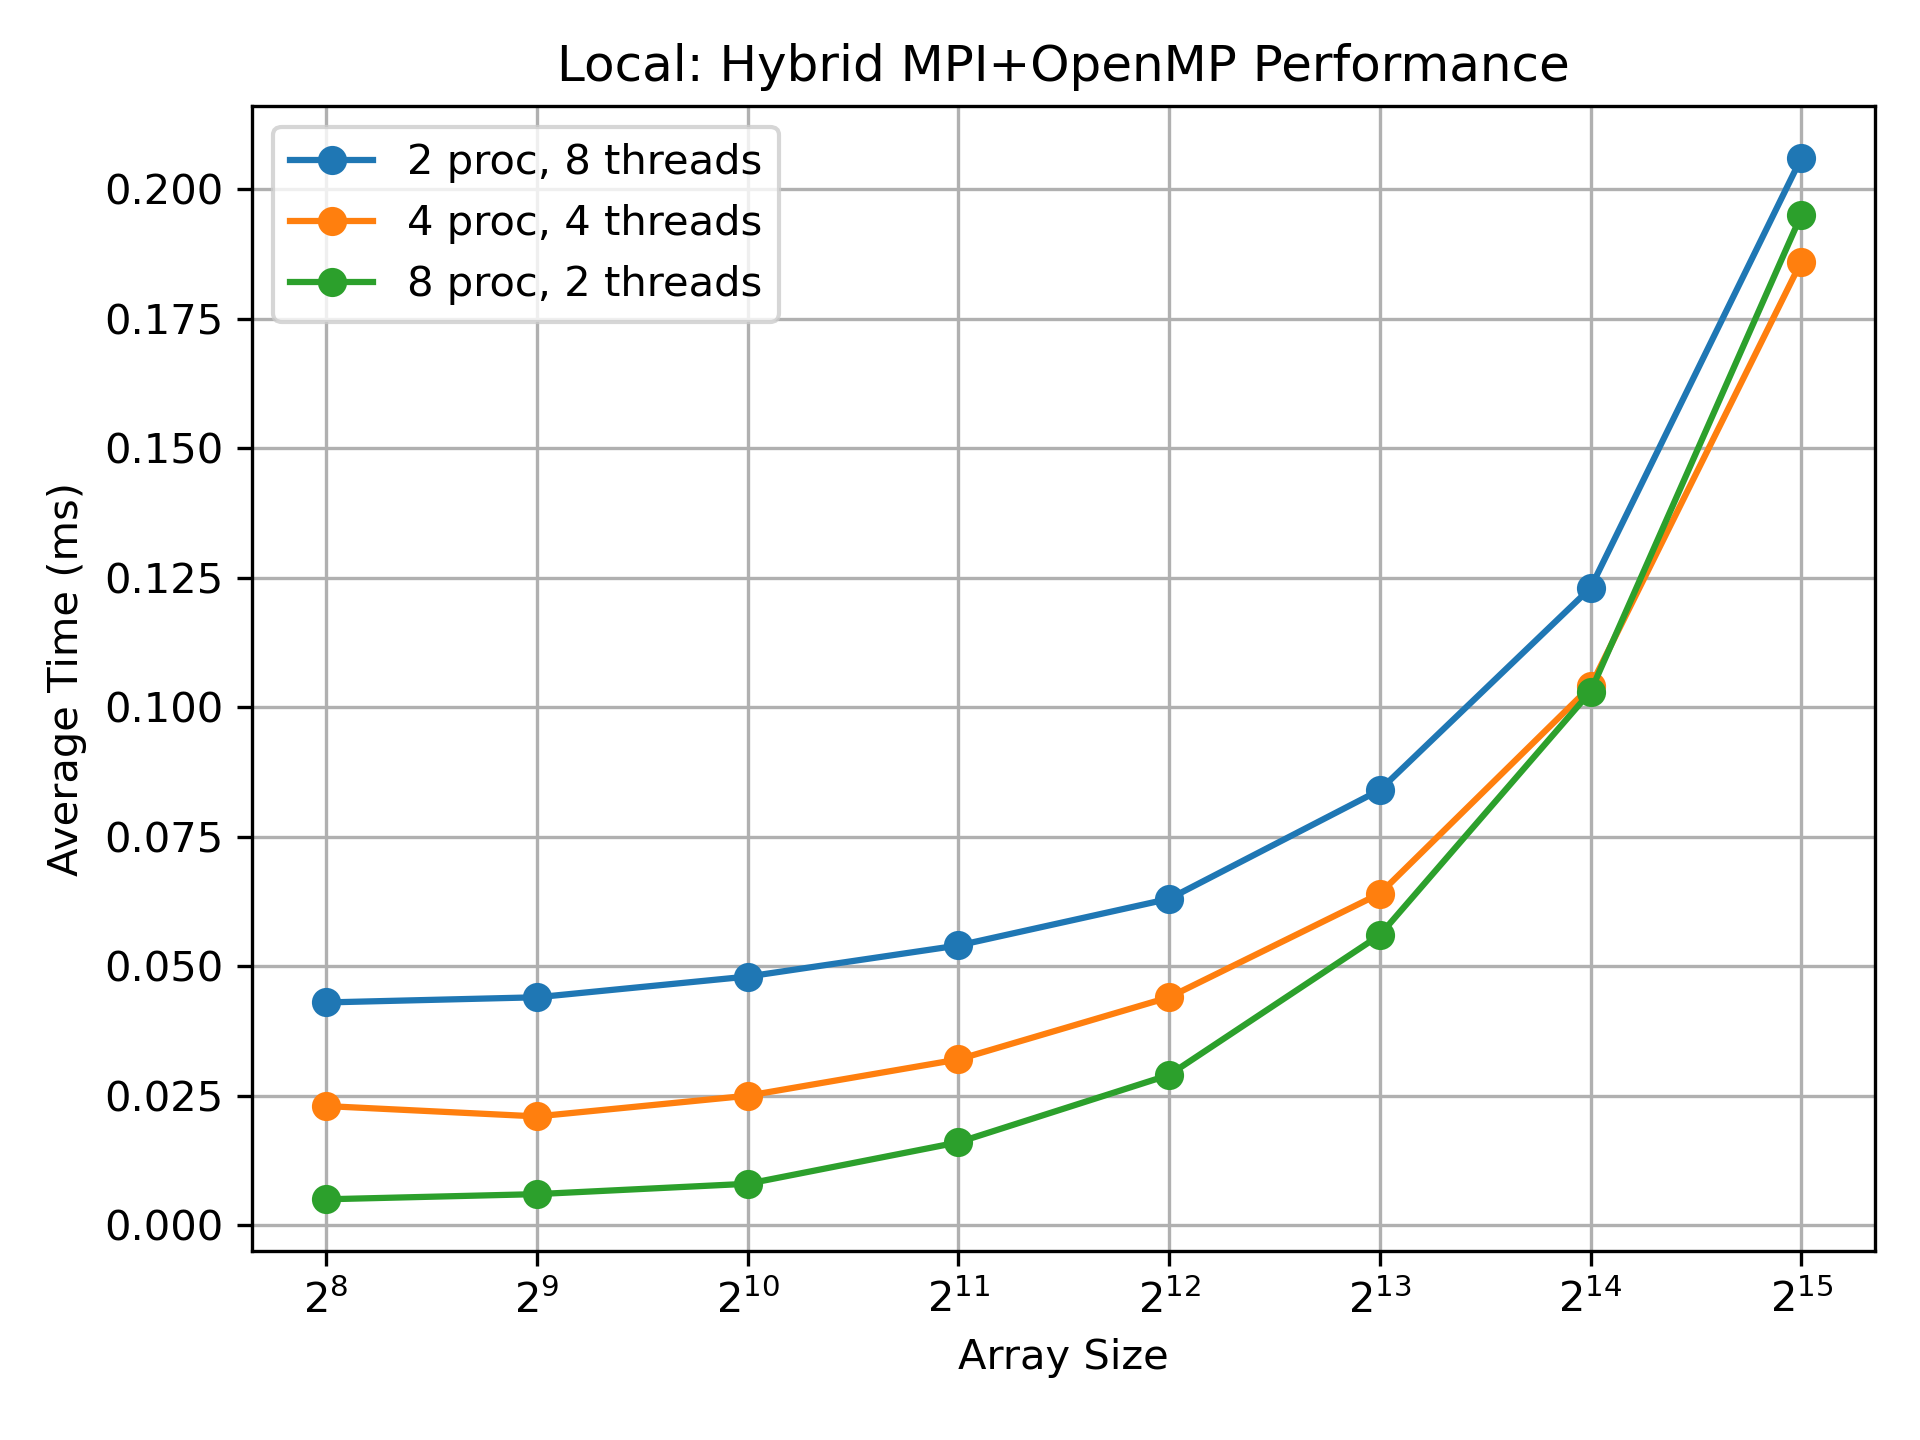
\includegraphics[width=\textwidth]{./images/localq7.png}
  \caption{Varied process$\times$thread configurations run locally}\label{fig:localq7}
\end{subfigure}%
\caption{Figures depicting the duration in seconds associated with varying process$\times$thread configurations on KNL server and local system}
\label{fig:gq7}
\end{figure}

Figures \ref{fig:knlq7} and \ref{fig:localq7} show the performance of numerous process and thread configurations (2 processes with 8 threads, 4 processes with 4 threads, and 8 processes with 2 threads) on the KNL system as well as my local system.
The figures compare the performance as the size of the array scales exponentially following a log base 2 pattern, with the smallest size being $2^8$ and the largest being $2^{15}$.
The tests were run via the \texttt{run.sh} script present in the Appendix in Code Block \ref{a:runq7}.
The script varied the array sizes and the process/thread configuration.
The code presented in Code Block \ref{q7:hybrid} iterated through the loop 100 times and retrieved the average time via \texttt{MPI\_Wtime()}; the timer overhead was also deducted accordingly.
The timing was done within the \texttt{.c} file and always after the \texttt{MPI\_Init()} function but before the array was filled and up until before any printing or logging took place.
As is expected, as the array size increases, all iterations take longer.
I extended this simulation locally to see how it would perform as my machine is capable of producing results quicker, and once the array size reaches anything beyond $2^{17}$, the differences are largely indistinguishable.
The plot of that data can be seen in Figure \ref{fig:bigq7}.
Despite this, these plots do point towards the fact that the implementations favouring MPI processes (8 processes by 2 threads and 4 processes by 4 threads) are more efficient at smaller array sizes as can be seen between data points $x=2^8$ and $x=2^{12}$.
This may be due to the fact that the OpenMP directive incurs additional overhead when compared to the associated MPI overhead.

\begin{figure}[H]
\centering
    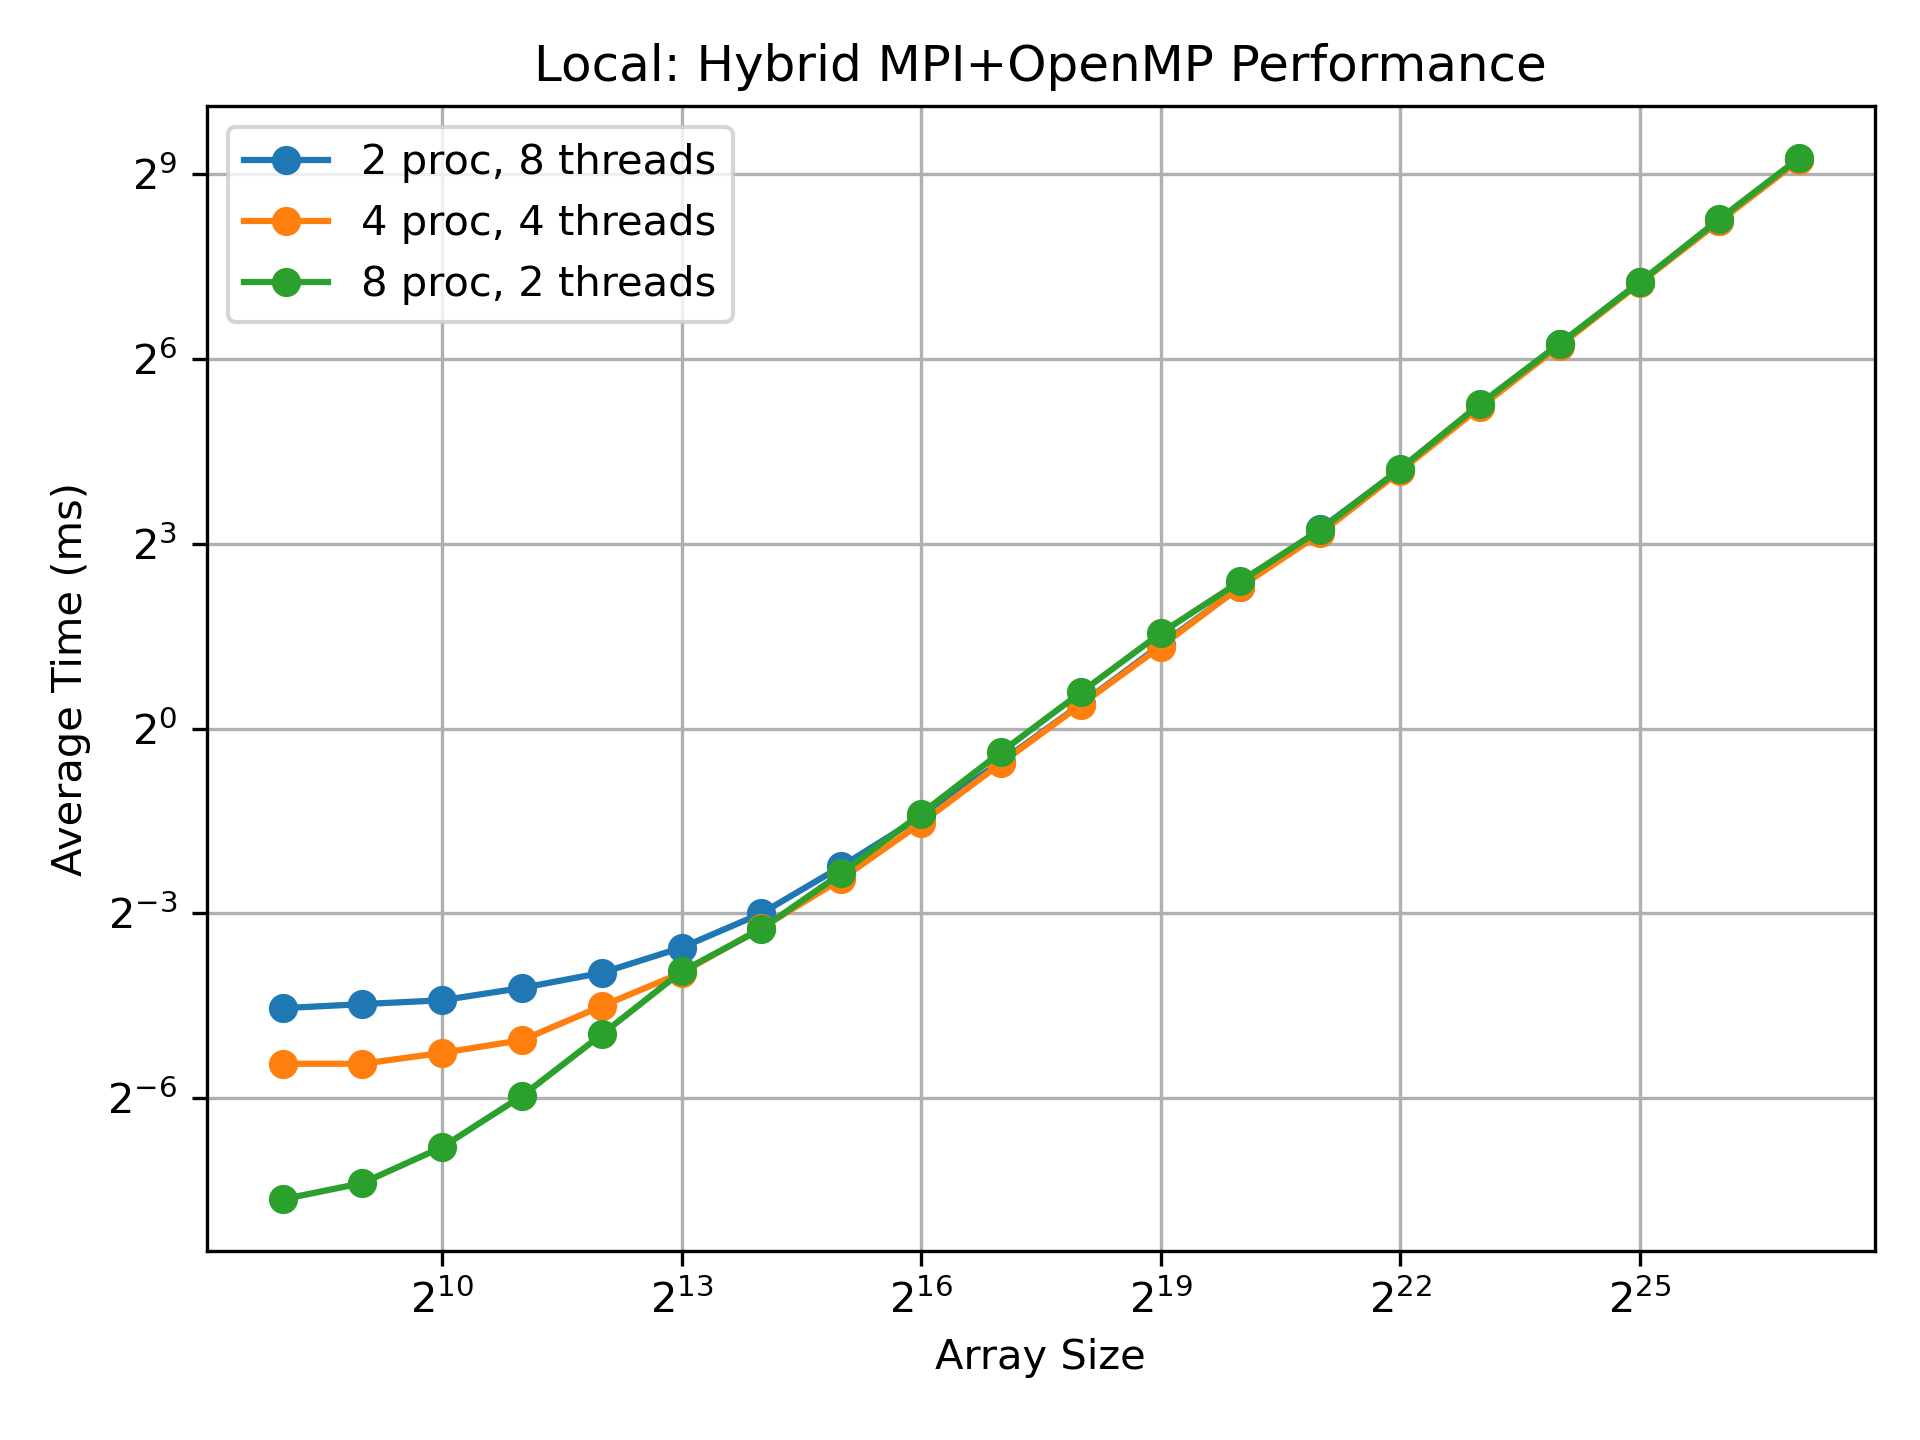
\includegraphics[width=0.5\textwidth]{./images/bigq7.png}
\caption{Graph depicting the duration in seconds associated with varying process$\times$thread configurations on my local machine}
\label{fig:bigq7}
\end{figure}

The output for the code can be found in Figure \ref{fig:q7} with the exception of the hybrid model, which for the sake of brevity is omitted as it was looped 100 times for analysis purposes and had varying array sizes.
As such, this is also some of the only code that isn't run via a \texttt{Makefile}.
The output presented was run with 8 processes and a fixed \texttt{srand} seed to ensure all iterations were correct.
\begin{figure}[H]
\centering
    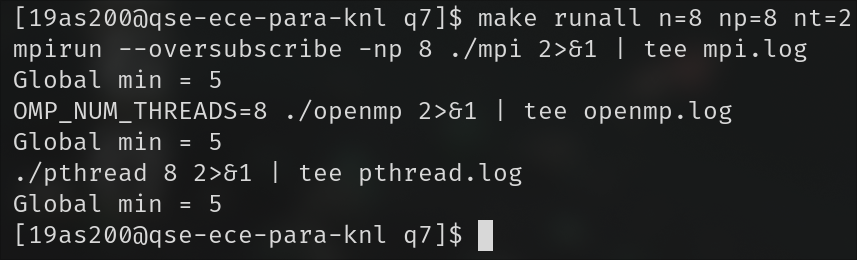
\includegraphics[width=0.5\textwidth]{./images/q7.png}
\caption{Output for question 7}
\label{fig:q7}
\end{figure}

\newpage
\section*{Q8:}

Code Blocks \ref{q8:mpiS} and \ref{q8:mpiD} present the question 8 code using MPI to calculate elements within the Mandelbrot set via static and dynamic scheduling respectively.
The output of the code can be seen in Figures \ref{fig:q8S} and \ref{fig:q8D}, with the two different colour schemes that generated the images themselves in Code Block \ref{q8:mpidisp}.
Only one of the colour schemes was utilized when generating the images, but both were included here for completeness.
Analysis of the performance of the code is in the Sub Section Analysis.
\lstinputlisting[language=C, caption=\centering{MPI code for question 8 static assignment}, label={q8:mpiS}]{../q8/mpi_static.c}
\lstinputlisting[language=C, caption=\centering{MPI code for question 8 dynamic assignment}, label={q8:mpiD}]{../q8/mpi_dynamic.c}
\lstinputlisting[language=C, caption=\centering{MPI code for question 8 dynamic assignment}, firstline=110, lastline=138, label={q8:mpidisp}]{../q8/mandelbrot-display.c}


\begin{figure}
\centering
\begin{subfigure}[t]{0.48\textwidth}
  \centering
    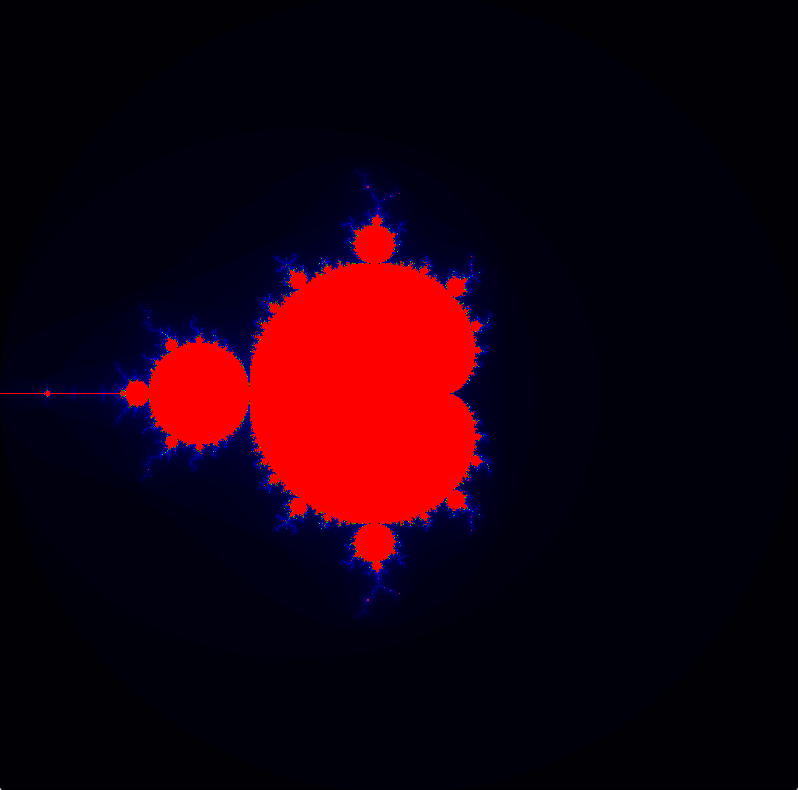
\includegraphics[width=\textwidth]{./images/static.png}
  \caption{static mandelbrot set coloured output}\label{fig:q8s}
\end{subfigure}%
\hfill
\begin{subfigure}[t]{0.48\textwidth}
  \centering
    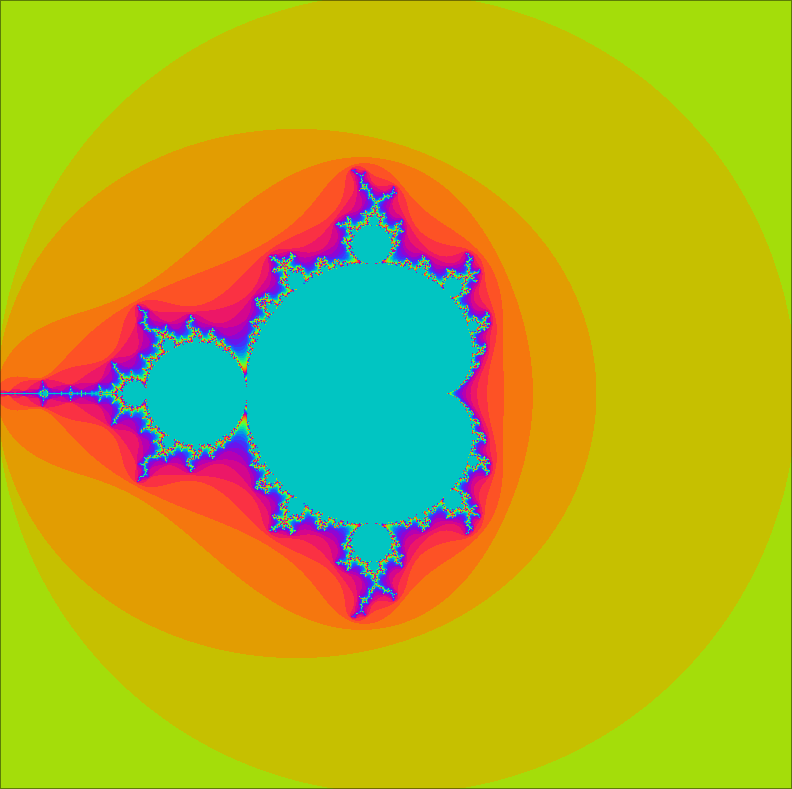
\includegraphics[width=\textwidth]{./images/dynamic.png}
  \caption{dynamic mandelbrot set coloured output}\label{fig:q8d}
\end{subfigure}%
\caption{figures depicting the coloured mandelbrot set at 800$\times$800 resolution}
\label{fig:outq8}
\end{figure}

\subsection*{Analysis:}

Similar to question 7, the code was run both on the KNL system and on my own local machine.
The graphs visible in Figure \ref{fig:q8S} and \ref{fig:q8D} were generated using the scripts in the Appendix. 
The code presented in Code Blocks \ref{q8:mpiS} and \ref{q8:mpiD} iterated through the loop 100 times and retrieved the average time via \texttt{MPI\_Wtime()}; the timer overhead was also deducted accordingly.
For both the dynamic and static code the timer was only started after the MPI init sequence to ensure only computation and intercommunication was timed.
Code Block \ref{a:runq8} of the Appendix was used to run numerous iterations with varying process counts, and Code Block \ref{a:plotq8} of the Appendix was used to plot the data.
The performance on the KNL system strays slightly from what would be expected, with the sequential code given to us in the assignment always taking longer than the MPI code. 
This is unexpected, as it should take less time than the statically or dynamically scheduled code utilizing 2 processes given there is overhead in the form of MPI initialization and communication.
The expected result can be seen in the locally run code in Figure \ref{fig:q8S}, where the baseline sequential code only performs better when the process count is 2.
Afterwards, the performance is as expected, where the more processes there are, the better the performance is. 
This holds true on both the KNL system and my local machine until 32 processes are reached at which point my system no longer has physical threads to assign to the processes, and as such, performance becomes worse when MPI begins oversubscription.
I am surprised to see that on both systems, the dynamically scheduled code is more performant all the time, I was expecting the 800 \texttt{MPI\_Send/Recv)()} operations used in dynamic scheduling to incur a larger overhead and thus perform worse than the statically assigned tasks, given that regardless of scheduling method, single \texttt{MPI\_Ints} are being sent.
It seems unlikely that this is an analysis error, as for each process count, 100 iterations were conducted.
It is more likely that this can be explained by the extra \texttt{malloc} and \texttt{realloc} operations leveraged by the static code, along with the possibility that different threads are much faster than others.
I would have been interested to see what varied work bundles beyond single rows would have resulted in for the dynamically scheduled code.

\begin{figure}
\centering
\begin{subfigure}[t]{0.48\textwidth}
  \centering
    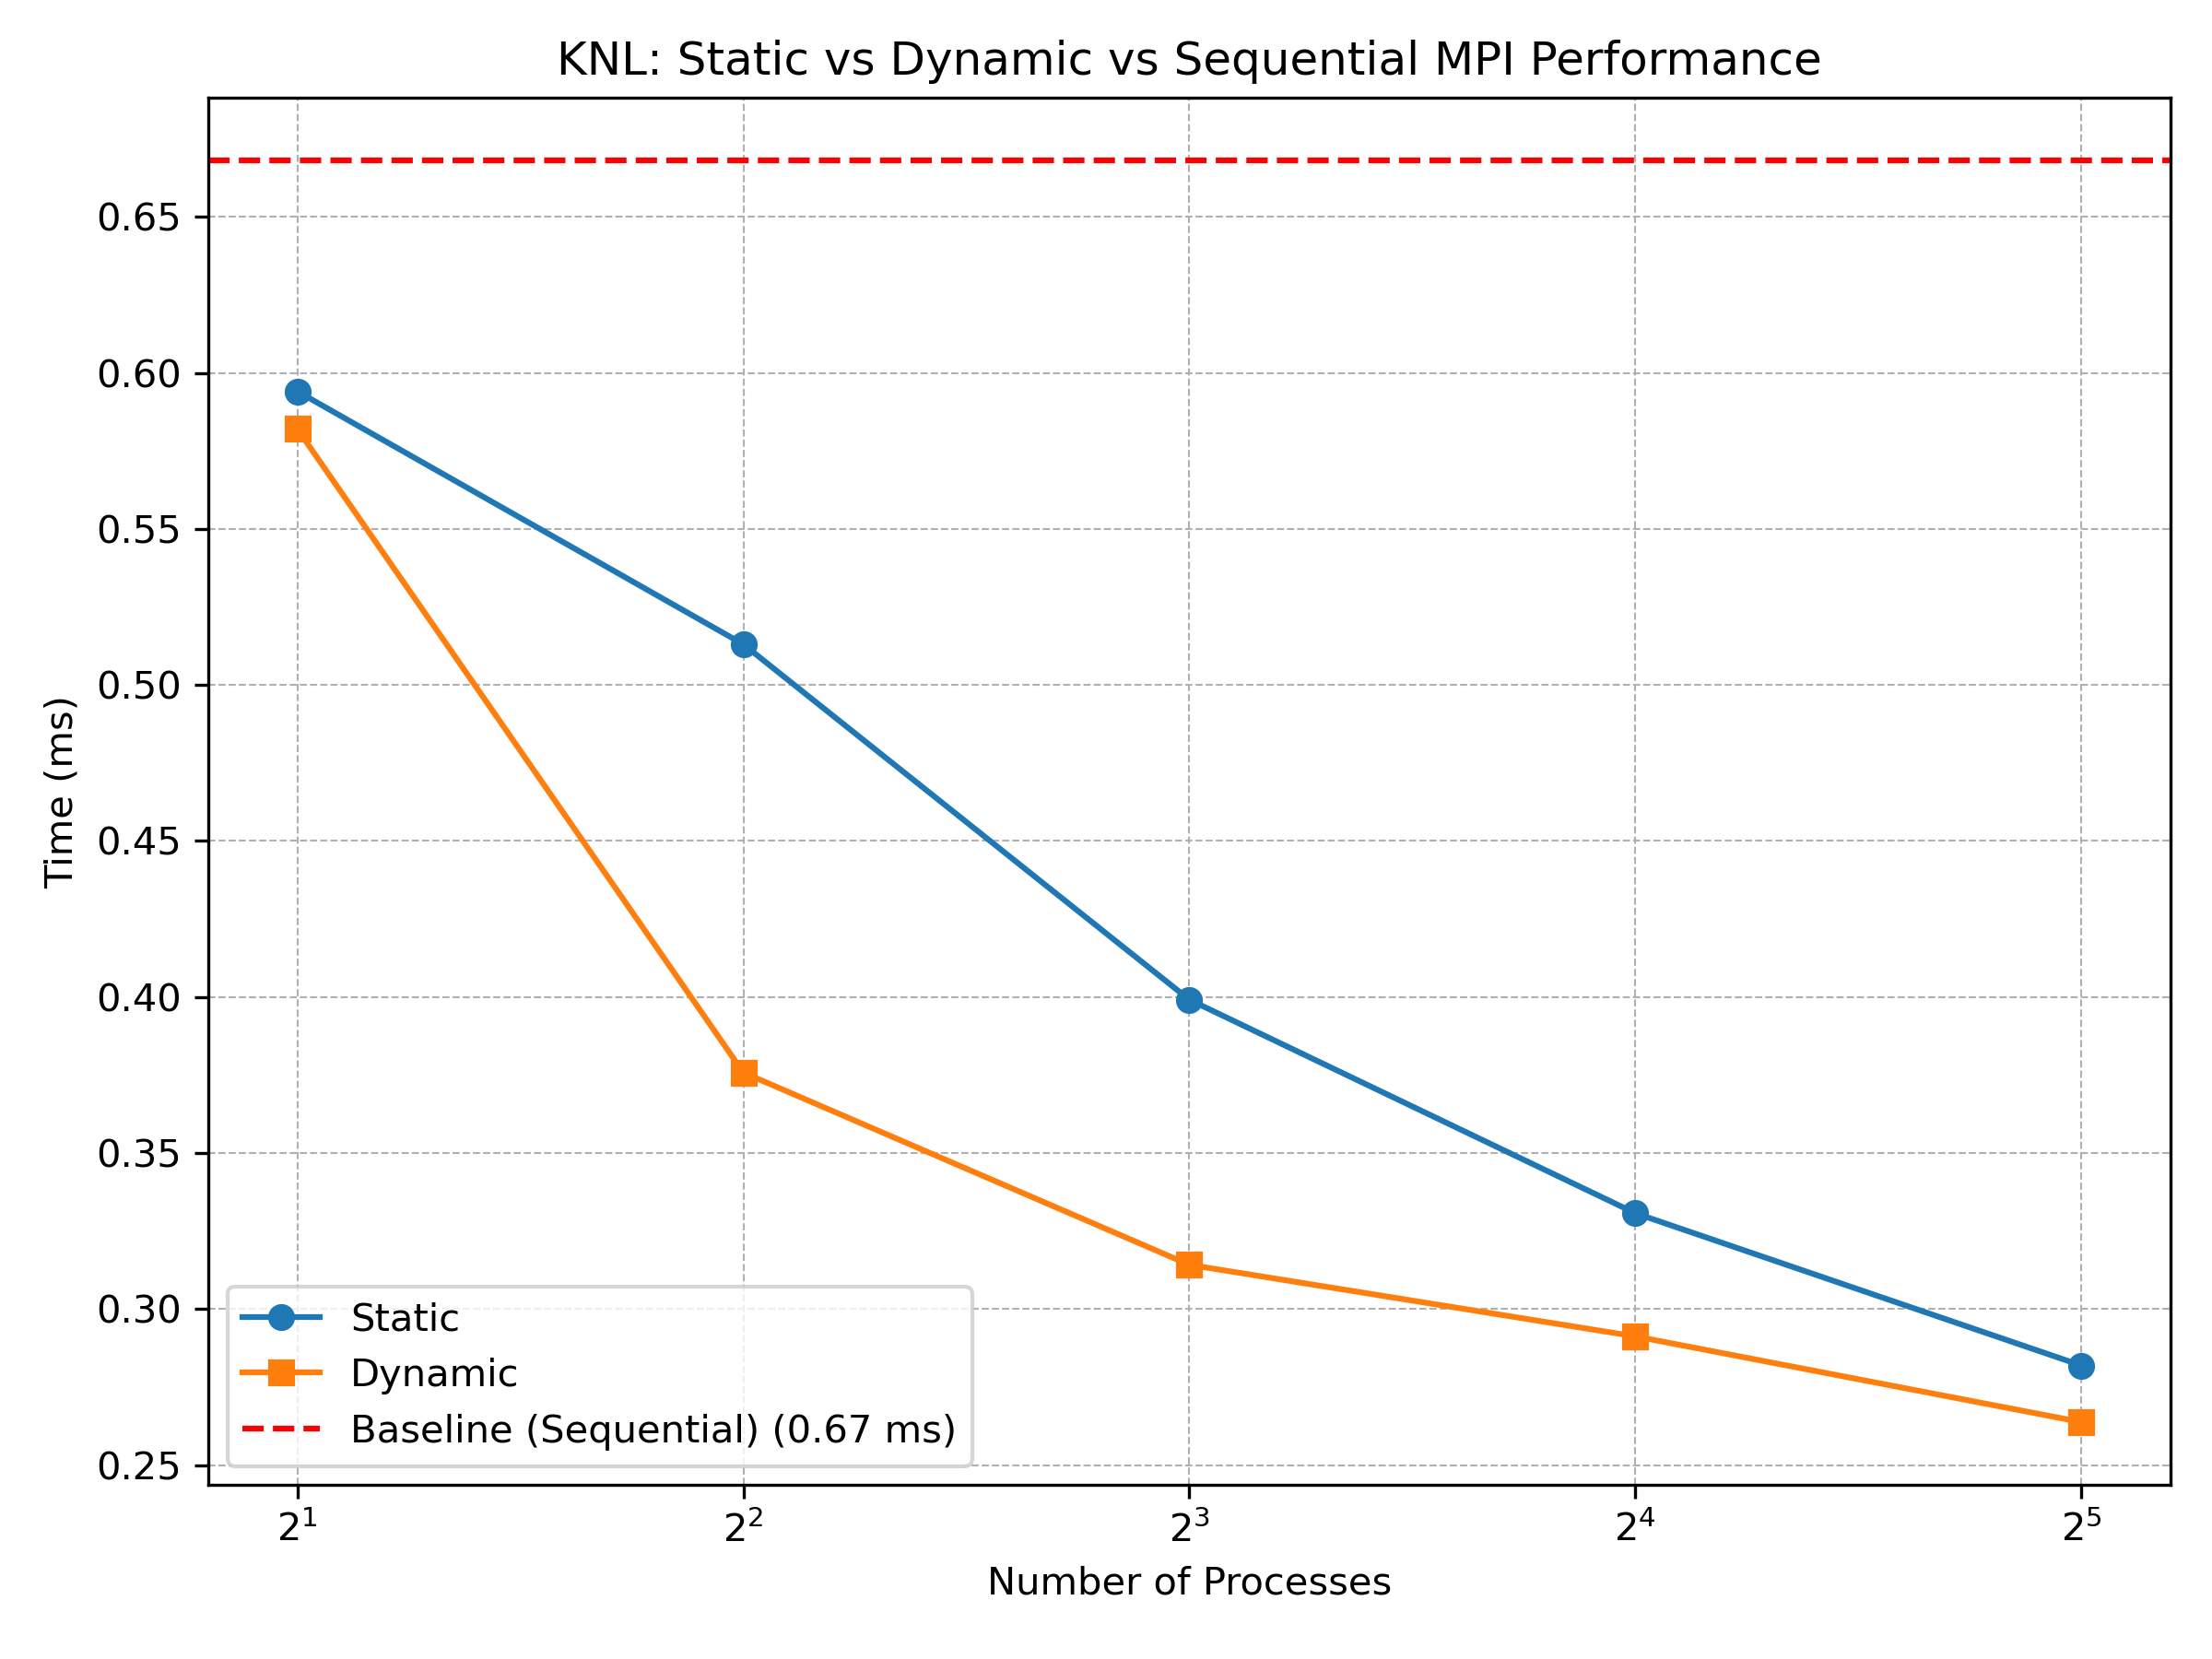
\includegraphics[width=\textwidth]{./images/knlq8.png}
  \caption{KNL performance graph}\label{fig:q8S}
\end{subfigure}%
\hfill
\begin{subfigure}[t]{0.48\textwidth}
  \centering
    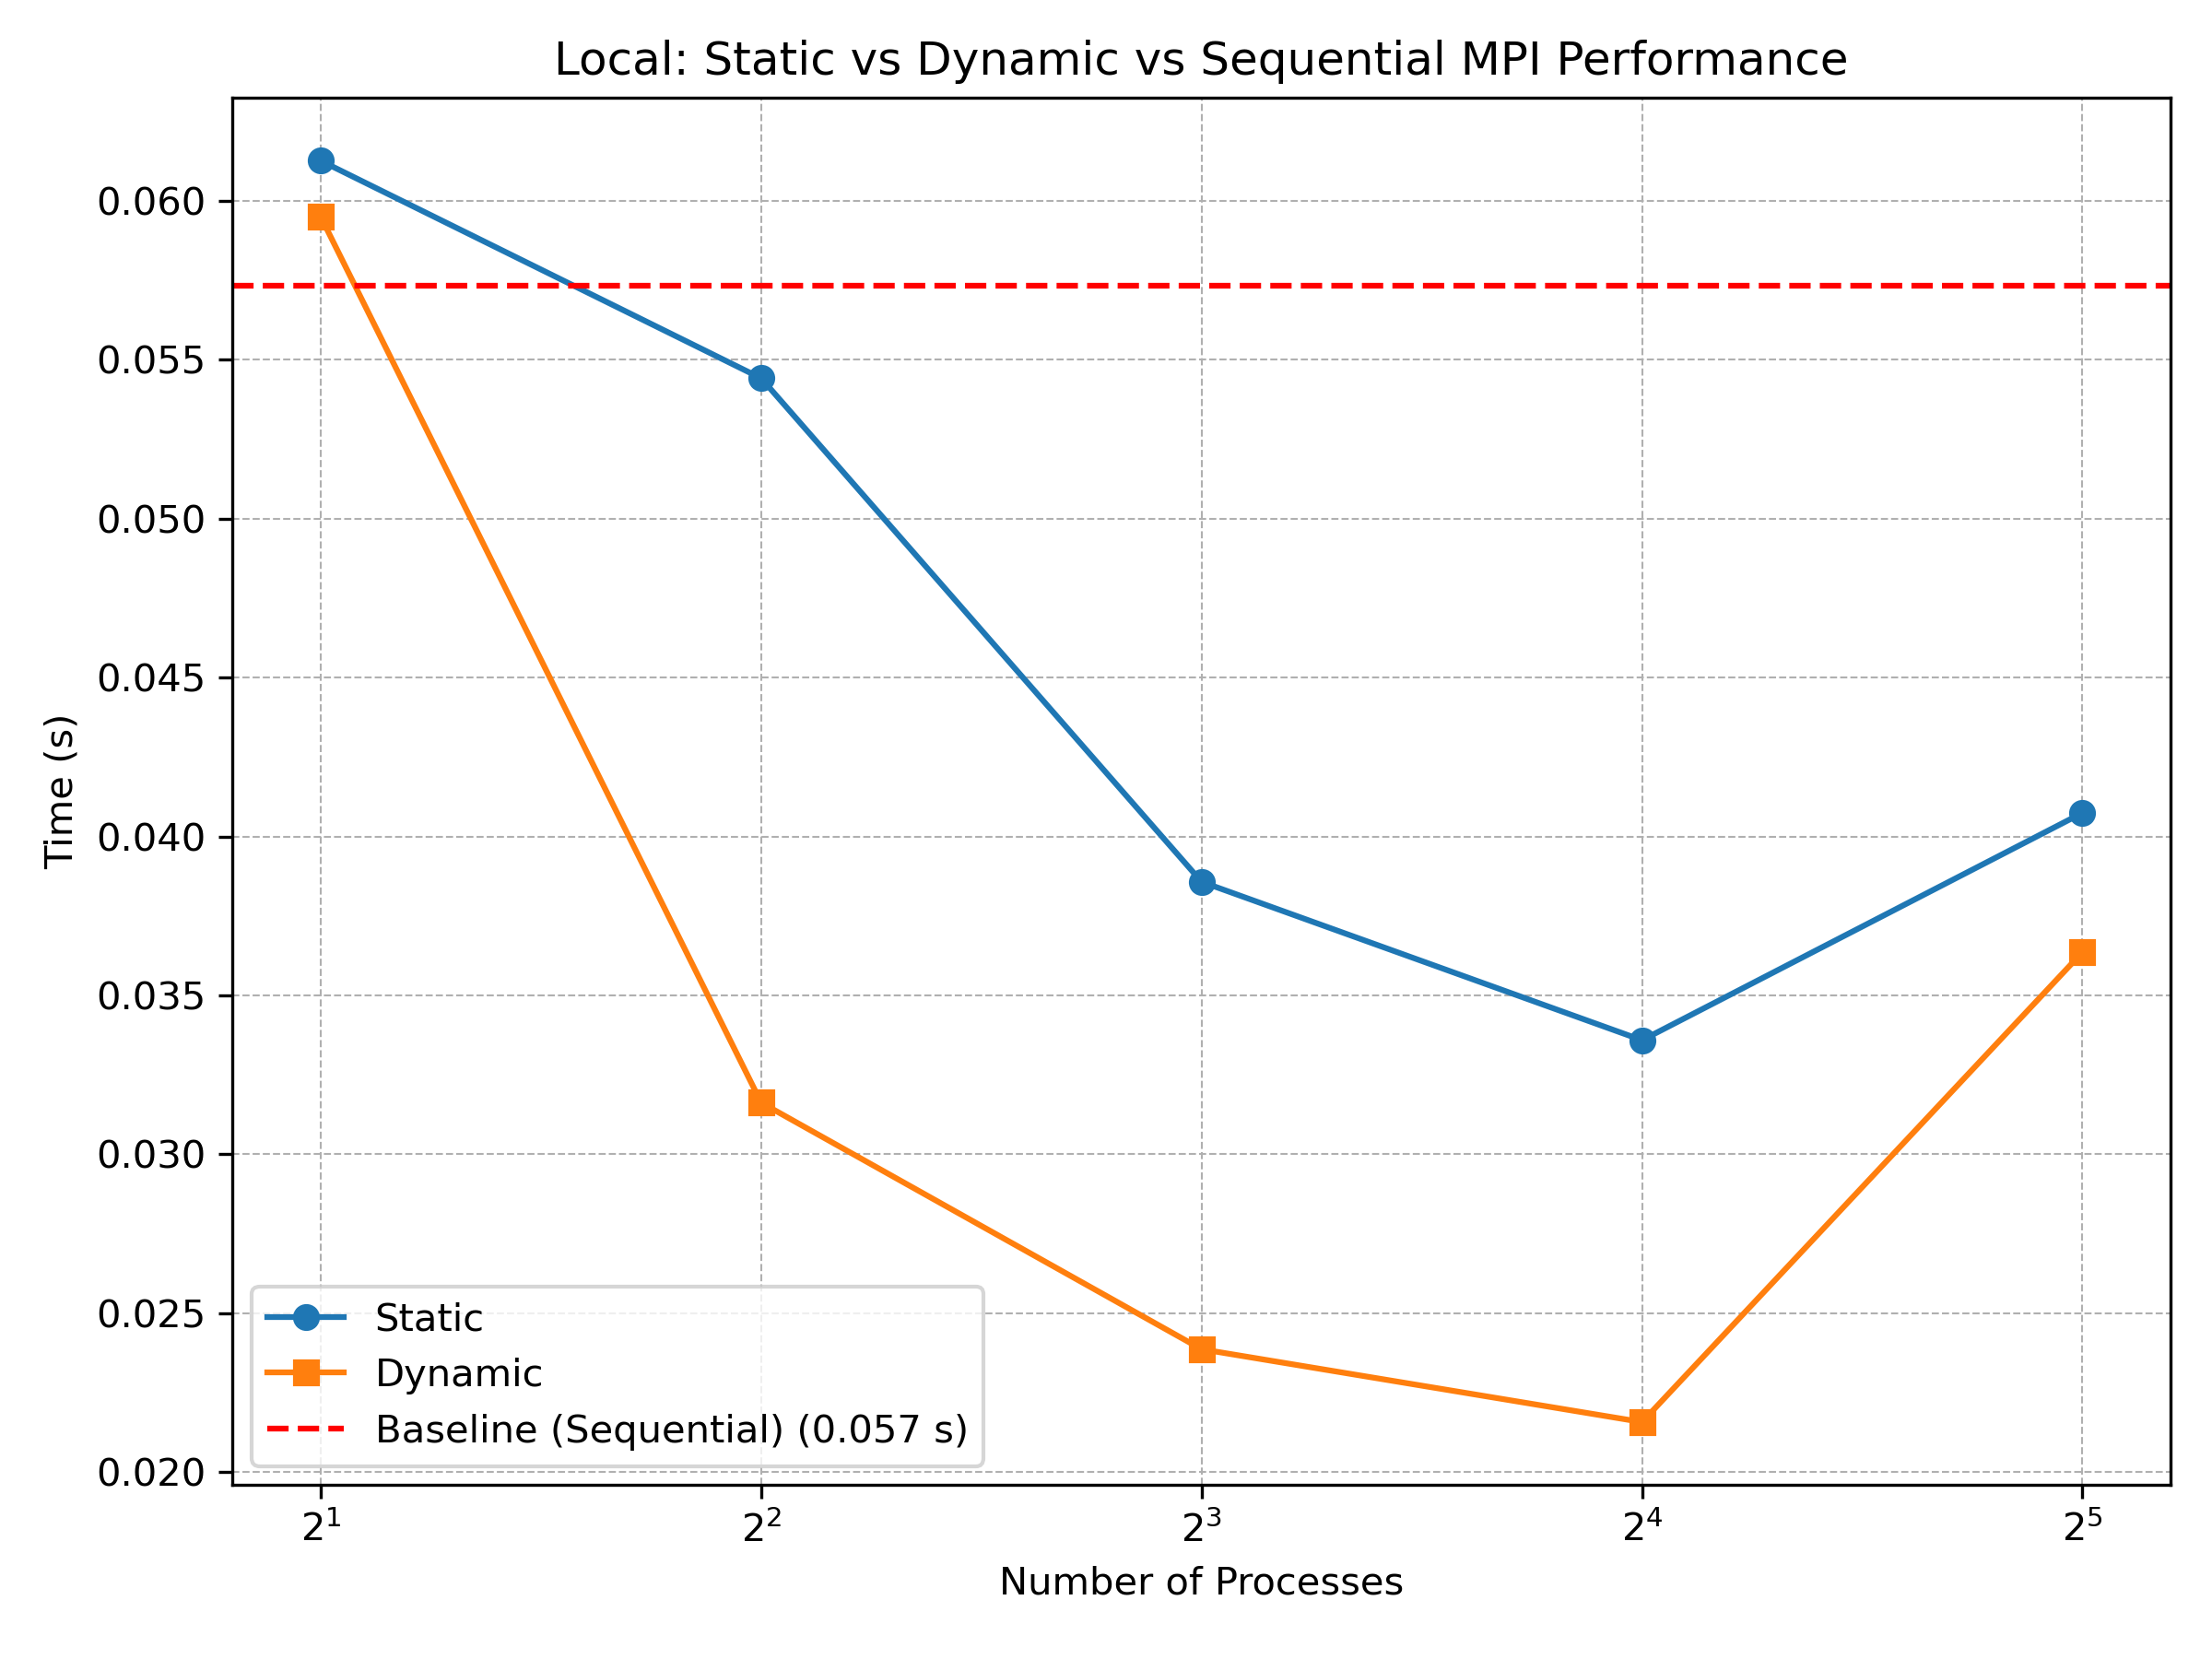
\includegraphics[width=\textwidth]{./images/localq8.png}
  \caption{Local performance graph}\label{fig:q8D}
\end{subfigure}%
\caption{Graphs depicting difference in performance between sequential (1 process) and statically\/dynamically scheduled MPI code at a variety of process counts (2-32)}
\label{fig:q8}
\end{figure}

\clearpage

\section*{Q9:}

Code Block \ref{q9:mpi} presents the question 9 code using MPI to compute the sum of 1000 numbers.
The output of the code can be found in the Figure \ref{fig:q9}.
The Code was run with 8 threads, but is modular and functions with any number of processes that are powers of 2 (due to the way the binary tree is navigated).


\lstinputlisting[language=C, caption=\centering{MPI code for question 9}, label={q9:mpi}]{../q9/mpi.c}

\begin{figure}[H]
\centering
    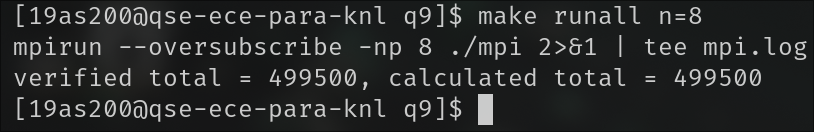
\includegraphics[width=\textwidth]{./images/q9.png}
\caption{Output for question 9}
\label{fig:q9}
\end{figure}

\clearpage
\begin{appendices}\label{Appendix}
  \lstinputlisting[language=make, caption=\centering{Makefile template used for all code}, label={a:make}]{../q1/makefile}
  \lstinputlisting[language=make, caption=\centering{Bash script used to vary process, thread, and array size for question 7}, label={a:runq7}]{../q7/run.sh}
  \lstinputlisting[language=make, caption=\centering{Python script used to plot results for question 7}, label={a:plotq7}]{../q7/results.py}
  \lstinputlisting[language=make, caption=\centering{Bash script used to process counts for question 8}, label={a:runq8}]{../q8/run.sh}
  \lstinputlisting[language=make, caption=\centering{Python script used to plot results for question 8}, label={a:plotq8}]{../q8/results.py}

\end{appendices}

\end{document}
